\chapter{\label{ch:2-bkgnd}Background}

\minitoc

This chapter describes fundamental concepts and gives literature review about research topics that are involved in this thesis. Topics covered include modeling and simulation, co-simualtion, parallel computing, scheduling in the context of parallel computing, and parallelization approaches related to (co-)simulation. 

\section{Modeling and Simulation}

The design of complex systems impose the study of their behavior before building them with the objective of allowing preliminary evaluation, tuning and possibly redesign of the solution. Simulation has proven successful in responding to this need and is becoming an indisputable step in the design process of complex systems. Simulation is an effective cost reducer since it allows to correct design errors before building the system. Simulation is performed by providing models which describe the behavior of the system and then running these models in order to produce the behavior of the simulated system on a computer.   

\subsection{Systems}

Before detailing the concepts and methods of modeling and simulation of systems, it is important to understand what is meant by a system. A system is defined as a set of interacting parts which form a complex whole. A system is characterized by the cohesion between its forming parts which operate as a whole towards a common goal. 

In order to have clearer understanding, the notion of a system should be conceived in the scope of the context that it is used in. In engineering domains, in addition to the definition given above, a system can be seen as an entity which receives inputs from the environment and produces outputs to the environment, and is characterized by an internal state. The state of the system is affected by the inputs that it takes, and, in turn, affects the produced outputs. Figure [ref] illustrates this view as usually found in block diagrams where $u$ represents the input of the system, $y$ the output, and $x$ the internal state.

A kind of systems that falls within the scope of this thesis is known as Cyber-Physical Systems (CPS). CPS consist of a combination of tightly interacting computational elements and physical processes. The computational elements are called embedded systems or controllers and are used to control the physical processes. They are interfaced with the physical processes through sensors and actuators. The controllers run control software whose behavior is affected by the physical process. Areas where CPS can be found are as important as automotive, aerospace, manufacturing, transportation and many others. The diversity of the involved disciplines makes the process of building CPS challenging, costly and time consuming.

\subsection{Modeling}

Modeling a system consists in creating a mathematical abstraction of its behavior. The first step is to choose a modeling formalism. This choice depends on the properties of the system, the objective of the simulation, and the aimed level of detail in the simulation. For instance, models can be built using continuous-time variables to represent continuous dynamics of a physical process. Such mathematical models consist of a set of differential equations which describe the continuously changing physical quantities of a process such as electrical circuits, fluid dynamics, chemical reactions, etc. Other systems feature a behavior which evolves between a finite set of states. These systems can be modeled as discrete event systems using formalisms such as DEVS (Discrete Event System Specification), Statecharts, or Petri nets. Finally, hybrid modeling allows the modeling of systems with both continuous variables and discrete states. In other words, the system jumps between discrete states and while it is in a certain state, it features a continuous behavior, i.e. its quantities change continuously. 

In this thesis, we focus on the the modeling of dynamical systems using differential equations. A differential equation expresses a variable as a function of its derivatives. In the modeling of dynamical systems, the variables are the physical quantities and the derivatives express their rates of change. A differential equation is called Ordinary Differential Equation, abbreviated ODE, if it involves ordinary derivatives of the variables with respect to an independent variable (usually the time in the modeling of dynamical systems).  Equation \ref{eq:ode} is an ODE where $x$ is the vector of the dependent variables of interest called the state variables, $\dot{x} = \frac{dx}{dt}$ is the vector of the time derivatives of the state variables, $t$ is the time (the independent parameter), and $f$ is a given function.

\begin{equation}
\dot{x} = f(x,t)
\label{eq:ode}
\end{equation}

In contrast, a differential equation is called Partial Differential Equation, abbreviated PDE if it involves unknown functions and their partial derivatives. Equation \ref{eq:pde} shows such PDE where $x_1,x_2,\dots, x_n$ are the parameters, $y=y(x_1,x_2,\dots, x_n)$ is the unknown function, and $f$ is a given function.

\begin{equation}
f\biggl(x_1,x_2,\dots, x_n,y,\frac{\partial y}{\partial x_1},\frac{\partial y}{\partial x_2},\dots,\frac{\partial y}{\partial x_n}\biggl)=0
\label{eq:pde}
\end{equation} 

A Differential Algebraic Equation, abbreviated DAE, is a system of equations which involves algebraic equations in addition to differential equations. A DAE can be written in the form shown in equation \ref{eq:dae} where $f$ represents differential equations involving derivatives of variables and $g$ represents algebraic equations which do not contain derivatives.

\begin{equation}
\begin{aligned}
&0 = f(\dot{x},x,t)\\
&0 = g(x,t)
\end{aligned}
\label{eq:dae}
\end{equation} 
  
In this thesis, we are particularly interested in modeling dynamical systems using ODEs. Typically, such systems are hybrid dynamic systems modeled using hybrid ODEs. These systems exhibit continuous behavior interspersed with jumps triggered by some events. There are two kinds of events: Events which occur at a particular instant in time are called time events. The other kind of events, called state events or zero-crossing, arise as a result of the value of a state variable crossing a specific threshold. Time events are easier to handle than state events since they occur at known instants in time. A classic example of such hybrid dynamic systems is the bouncing ball model where a ball is dropped from a certain height above the ground. The ball falls with a velocity subject to gravity and bounces when it hits the surface. Equation \ref{eq:bb} gives a hybrid system of equations which describe the behavior of the bouncing ball where $x$ is the position of the ball (height), $v$ its velocity, $g$ the gravity constant, and $\gamma$ the coefficient of restitution.

\begin{equation}
\begin{aligned}
&\dot{x} = v\\
&\ddot{x} = -g\\
&\dot{x} := -\gamma \dot{x} 
\end{aligned}
\label{eq:bb}
\end{equation}  

The bouncing ball model exhibits a continuous behavior when $x > 0$ and discontinuities occur at bounces, i.e. when $x = 0$, where the velocity of the ball is inverted and scaled down by a factor equal to $\gamma$. In other words, the motion of the ball changes from downward to upward. Figure %\ref{fig:bbtrajectory} 
shows the trajectory of the ball. This hybrid dynamic system can be modeled using a hybrid automaton as shown in figure %\ref{fig:bbautomaton}.

%\begin{figure}
%
%\label{fig:bbtrajectory}
%\end{figure}

%\begin{figure}
%
%\label{fig:bbautomaton}
%\end{figure}

\subsection{Simulation}

Given a model of the system under study, the simulation consists in running this model in order to produce and plot, on a computer, the time varying values of the quantities of interest. This data is used in order to assess different aspects about the functioning of the system. Technically speaking, running a model which consists of a set of ODEs means solving these equations. In practice, it is not possible to find the solution of such equations analytically which imposes the use of numerical methods to solve them. Such numerical methods, called solvers, are based on the principle of discretization of the time $t$. This means that the values of the state variables $x(t)$ of an ODE in the form of equation \ref{eq:ode} evolve between discrete points of time, called \textit{time steps}, $(t_k, t_{k+1}, \ldots)$ instead of an evolution in continuous time $t \in \mathbb{R}^+$. The distance between two time steps is called the \textit{integration step size}. The smaller is the integration step size, the more accurate is the numerical resolution of the equations, i.e. the closer it is to the exact solution. However, reducing the integration step size requires more computations and thus slows down the execution of the solver. A tradeoff has to be made according to the desired quality and computation speed.

The discretized time can be written as: $t_k = k \times h$ where $h$ is the integration step size. The solver computes a sequence: $x_{k+1} = F(x_k,t_k)$ where $x_k$ is the value of the variable $x$ at $t_k$, the $k^{th}$ time step. $F$ is the solver or the integration function. Starting from the initial time $t_0$ and having the initial condition $x_0$, which is the value of $x$ at time $t_0$, the numerical resolution consists in computing approximate values of the quantity $x$ repeatedly with respect to the discretized time. The time step $h$ has to be chosen in such a way that the dynamics of the simulated system are well captured. When the system exhibits dynamics heterogeneity, e.g. fast transients with slow evolution of the state variables, a fixed time step becomes less efficient. It is therefore  more efficient to use a variable time step. A solver with variable step controls the step size using a feedback loop on the error. The step size is adapted according to an estimation of the error. 

Solvers are characterized by a number of properties (e.g. order, explicit/implicit, fixed/variable integration step size, \ldots) which should be taken into consideration when choosing a solver for a specific problem. Overall, it is always desirable to choose a solver that is reliable, robust and fast.

\subsection{Co-simulation}

Complex systems may involve heterogeneous interacting parts. For instance, In a CPS, the controlled physical process constitutes a multi-physics system and is modeled in the continuous-time domain using (hybrid) Ordinary Differential Equations (ODEs). On the other hand, because they are implemented on embedded computers, numerical laws that control the physical process are modeled in the discrete-time domain. For such systems, it becomes necessary to do the modeling on the subsystem level, usually without a complete view about the the rest of the system. Models are then coupled together in order to perform simulation at the system level, known as co-simulation. In co-simulation, the different models are simulated in a black-box fashion and an orchestration of their interactions has to be ensured. The interactions between the involved models consist in data exchange.

Co-simulation is an alternative approach to monolithic simulation where a complex system is modeled as a whole using differential equations and simulated by numerically solving these equations. Co-simulation has a number of advantages over the monolithic approach. It allows modeling each part of the system using the most appropriate tool instead of using a single modeling software. Also, it allows a better intervention of the experts of different fields at the subsystem level. Furthermore, co-simulation facilitates the upgrade, the reuse, and the exchange of models. 

In co-simulation of models based on ODEs, the equations of each model are integrated using a solver separately. Models exchange data by updating their inputs and outputs at fixed points in time called \textit{communication steps}. The distance between two communication steps is referred to as communication step size and denoted $H$. The communication step size associated with a model is greater or equal to the integration step size of the models and defines the rate of communication (data exchange) of this model. Figure shows the evolution of time and data exchange between two models A and B. In this example, the equations of model A are solved using a fixed step size $h_A$ whereas the equation of model B are solved using a variable step step $h_B$. The communication step size is considerably larger than both integrations step sizes, allowing fast progress of the integration of the equations by restricting the data exchange to occur at communications steps only. Between communications steps, each model considers that the values of data produced by the other models are held constant. Another alternative is to estimate these values by employing extrapolation techniques.

For larger co-simulations involving more models, different communication step sizes may be associated with different models. In this case, we talk about multi-rate co-simulation.

In the context of CPS which contain embedded systems controlling physical processes, different kinds of co-simulation, presented hereafter, can be performed depending on the stage of the controller design.

\subsubsection{Model-in-the-Loop}

Model-in-the-Loop (MiL) co-simulation is performed at an early stage of the controller design. In MiL, the model of the controller is included with the model of the controlled physical process in a co-simulation is used to test and validate the functioning scenarios of the controller. By using a system model, MiL aids in the design of control algorithms and also the investigation of design concepts. Once the functions of the control algorithm are specified, the controller software can be implemented.

\subsubsection{Software-in-the-Loop}

Once the controller model is validated, it can be implemented to perform Software-in-the-Loop (SiL) co-simulation. The controller software code can be generated from the controller model. It is then integrated with the simulated models and executed on the computer that runs the simulation. SiL is an inexpensive approach to perform realistic tests of the controller’s performance without the need for using a special hardware. It is common to move back and forth between the MiL and the SiL stages to make necessary rectifications if design flaws are detected.

\subsubsection{Hardware-in-the-Loop}

After the verification of the controller software, the next stage consists in performing Hardware-in-the-Loop (HiL) co-simulation. In HiL, the controller software is implemented on the real hardware (e.g. Electronic Control Unit) which is connected to the computer that runs the simulation of the physical process. HiL must run in real-time in order to imitate the real interactions between the controller and the physical process. It can ensure reliable tests of the controller and thus shortens the development time and reduces the costs. If any problems are detected, one can go back to SiL or MiL stage to make necessary corrections.

Figure gives a v-cycle view of the different stages of co-simulation performed as part of the process of controller design.


\subsubsection{The Functional Mock-up Interface Standard}

The Functional Mock-up Interface (FMI) is a tool-independent and open standard designed in the context of the MODELISAR project and is currently developed and maintained by the Modelica Association\footnote{https://www.modelica.org/association/}. FMI standard was developed in order to facilitate the co-simulation of dynamical systems, such as CPS. It provides specifications in order to enable the exchange and the co-simulation of heterogeneous dynamical models that may be developed by different tools. A modeling tool that supports FMI can export a model as a Functional Mock-up Unit (FMU) which can be used in co-simulation environments. FMI defines interfaces for the involved models to allow their co-simulation.

%\begin{figure}[h]
%\centering
%\captionsetup{justification=centering}
%\includegraphics{figures/fmifigure}
%\caption{Vision on how FMI can be used in the automotive domain\footnotemark.} 
%\label{fig:fmifigure}
%\end{figure} 


An FMU is a package that encapsulates different files:

\begin{itemize}
\item An XML file that contains among other data the definition of the different variables of the models and the description of the dataflow between these variables. 
\item Model functions: Standardized C-functions that are used to create instances of the FMU and run them. The functions can be provided as platform dependent binaries (e.g. DLL files) or as C source code.
\item Documentation: Optional files that contain documentation about the model.
\end{itemize}

The FMI standard is organized in two parts:
\begin{itemize}
\item FMI for Model Exchange
FMI for Model Exchange specification provides interfaces and defines how model equations should be encapsulated in components. It allows solving each model independently using custom solvers. Accessing and computing the equations is done through standardized function calls.

\item FMI for Co-Simulation:
FMI for Co-Simulation specification defines interfaces between a master algorithm and slave models. It is intended to couple different simulators (models with their solvers) in a co-simulation environment.
\end{itemize}
Figure shows the state machine of the supported calling sequences from a master algorithm to a slave.

%\begin{figure}[h]
%\centering
%\captionsetup{justification=centering}
%\includegraphics[scale=0.6]{figures/callingsequence}
%\caption{Calling sequence of Co-Simulation C functions in form of an UML 2.0 state machine} 
%\label{fig:callingsequence}
%\end{figure}  


%\begin{figure}[htb]
%\centering
  %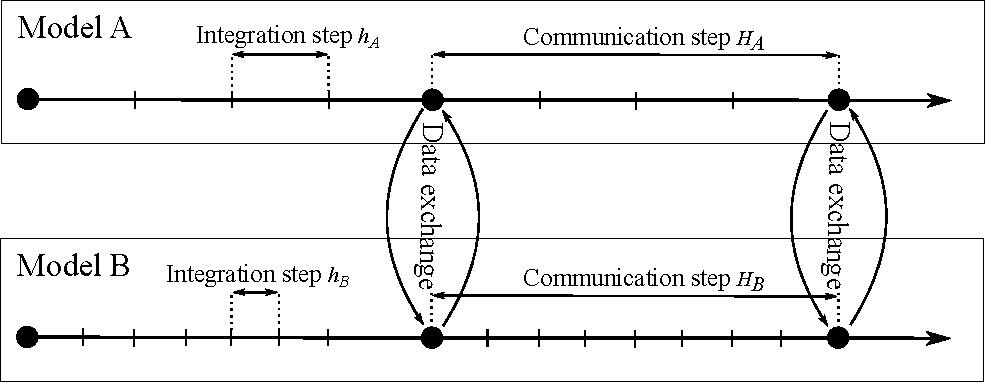
\includegraphics[scale=0.7]{figures/Co-Simulation}
%\caption{Evolution of time and data exchange between two models during co-simulation}
%\label{fig:cosim}
%\end{figure}

\subsection{Co-simulation with Real-time Constraints}

In the design process of complex systems, it is often necessary to test the behavior of the system as it would be produced by the real system. Therefore, the simulation is executed with real-time constraints such that the progress of the simulation time matches the real-time. For example, if temperature takes three minutes to reach $25$°, the simulation has to take three minutes as well. Similarly, a co-simulation with real-time constraints has to be executed with the same rate of the real-time.

A typical application of real-time co-simulation is HiL. The key advantage of real-time co-simulation is that it allows testing the controller under real-like conditions even if the physical process is not available. Many HiL solutions are developed in such a way to work using special dedicated hardware that provides an execution fast enough to ensure real-time constraints. Other solutions tend to enable real-time co-simulation using general purpose computers equipped with Real-Time Operations Systems (RTOS).

Roughly speaking, the difference between real-time simulation and non real-time (offline) simulation is related to the notion of results validity. For offline simulation, one seeks to obtain results as soon as possible. The validity of the the results depends only on their numerical accuracy. For real-time simulation, the validity of results depends on their numerical accuracy but also on their availability time, i.e. they have to be available within specific time bounds. If such bounds are missed, the results are considered invalid even if their values are correct from a numerical standpoint.

Figure [ref] illustrates the time evolution of a real-time simulation. During the resolution of the differential equations, the value of each variable $x$ is computed at every time step. The computation of $x_{n+1}$, the value of $x$ at time step $t_{n+1}$, cannot start before the value $x_n$ is computed as the computation of $x_{n+1}$ depends on the value of $x_n$. If the time required to compute the value of $x_{n+1}$ exceeds the step size, the real-time simulation constraints are violated which makes the simulation invalid. This is known as an \textit{overrun}.

\subsection{Languages and Tools for Modeling and Simulation}

Building models of systems can be done manually and than transformed into software using general purpose programming languages such as C. However, this approach is not efficient in practice, especially when the modeled system is complex and changes may be required in the model. Many tools and languages for modeling and simulation have been developed in order to facilitate and make the modeling and simulation more efficient. Such tools allow the user to specify an equation-based model in a straightforward manner and come with built-in solvers. Below, we present some tools and languages for modeling and simulation.

\subsubsection{xMOD}
xMOD\footnote{http://www.xmodsoftware.com/} is the modeling and co-simulation software developed by IFP Energies nouvelles. It supports FMI and provides an environment for the integration of heterogeneous models built by different parties using different languages and tools. xMOD can execute models embedding different solvers with different integration and communication step sizes. xMOD does not replace original modeling and simulation tools. Instead, it promotes and facilitates their coupling and existence.

%\begin{figure}[h]
%\centering
%\captionsetup{justification=centering}
%\includegraphics[scale=0.5]{figures/mipsxmod}
%\caption{Example of co-simulation models in xMOD.} 
%\label{fig:mips}
%\end{figure} 

\subsubsection{MATLAB Simulink}
Simulink\footnote{www.mathworks.com/products/simulink/}, developed by The Mathworks is a graphical modeling environment. Simulink is used in the  process of Model-Based Design of embedded systems. Models are built graphically in Simulink using block diagrams. In addition, Simulink is integrated in MATLAB which allows the incorporation of MATLAB algorithms in Simulink models. Finally, Simulink enables automatic code generation form models.

\subsubsection{Modelica}

Modelica is an object-oriented equation-based language for the modeling of complex physical systems developed by the Modelica Association. Modelica allows the modeling of physical systems by writing a set equations. Modelica adopts an acausal approach, i.e. the signal flow is not specified in the model. The simulator has to perform symbolic manipulations in order to define inputs and outputs and find an order of execution for these equations.

\subsubsection{Dymola}

Dymola\footnote{http://www.3ds.com/products-services/catia/products/dymola}, developed by Dassault Syst\`emes AB, is a modeling and simulation environment based on the Modelica modeling language. Dymola supports the FMI standard and allows interfacing with other tools such as Simulink

\subsubsection{Amesim}
Amesim\footnote{www.plm.automation.siemens.com/en\_us/products/lms/imagine-lab/amesim/} is a modeling and simulation software developed by Siemens PLM Software. Amesim can be used for the modeling and simulation of mechatronic systems. Amesim is based on the Modelica modeling language. It is oriented towards the modeling of complex physical systems instead of controller design. Amesim provides libraries containing collections of components that can be loaded and connected by the user to build models. For simulation, Amesim automatically selects a solver that is adapted to the problem.

\subsubsection{Hopsan}
Hopsan\footnote{https://www.iei.liu.se/flumes/system-simulation/hopsan?l=en} is a free multi-domain system co-simulation tool developed at the division of Fluid and Mechatronic Systems at Link\"oping university. Hopsan supports the FMI standard and model export to Simulink.
\section{Parallel Computing}

Parallel computing is a very important branch in the computing research and industry. It refers to the discipline that focuses on executing multiple computations simultaneously to solve one problem. Its basic idea is to divide a computing task into several sub-tasks that can be performed at the same time. From the beginning of the modern era of computing, computer software has been typically written for sequential execution. In order to solve a problem, an algorithm is designed as a sequence of instructions that are executed one after the other. In order to increase the computation power of computers, the dominant method was frequency scaling. If a processor's frequency is increased, it means that it can execute more instructions per clock cycle and thus can execute a sequential program faster. Moore's law predicted that the number of transistors in a processor would double approximately every two years \cite{moore:1965}. This prediction proved correct for many years. However, frequency scaling is facing technological limits and the last decade witnessed a wide shift to multicore processors among semiconductor manufacturers. Moore's law can be considered to be still accurate since more transistors are still integrated in chips, not for frequency scaling but to add more processing elements. The rise of multicore processors has caused the evolution of many parallel hardware and software technologies.

The main goal of parallel computing is to execute computer programs faster. The speedup obtained from the parallelization can be predicted using Amdhal's law \cite{amdahl:1967}. It states that for a program that is paralellized in order to be executed on multiple processors, the portion of the program that has to be executed sequentially will limit the speedup. The speedup is therefore not linear with the number of processors and probably adding more processors will not make the program run faster. The following formula gives the theoretical speedup computed using Amdahl's law.
\begin{equation}
S(n) = \frac{1}{(1-P) + \frac{P}{n}}
\end{equation}
$S(n)$ is the theoretical speedup, $P$ is the portion of the program that can be parallelized and $n$ is the number of processors. Figure \ref{fig:amdahl} shows the theoretical speedup of a program in function of the number of processors for different values of $P$. It shows for example that if $50\%$ of a program can be parallelized, the maximum possible speedup is 2, and if $95\%$ of the program can be prallelized, the maximum speedup is around 20.

%\begin{figure}[h]
%\centering
%\captionsetup{justification=centering}
%\includegraphics[scale=0.6]{figures/amdahlspeedup}
%\caption{Theoretical speedup computed using Amdahl's law for a program in function of the number of processors for different values of $P$.}
%\label{fig:amdahl}
%\end{figure} 

\subsection{Types of Parallelism}

Different kinds of parallelism exist: bit-level, instruction-level, data, and task parallelism.

\subsubsection{Bit-level parallelism}
Bit-level parallelism is the lowest level of parallelism and is related to the word size of the processor. If a 8-bit processor needs to perform computation on 16-bit data, it has to execute it in at least two steps, first on the 8 lower-order bits of the data and then on the 8 higher-order bits. Increasing the word size of the processor to 16 would allow the computation to be executed in one instruction. 

\subsubsection{Instruction-level parallelism}
Instruction-level parallelism allows the execution of more than one instruction per clock cycle if the instructions do not depend on each other. An example of instruction-level parallelism is instruction pipeline in which an instruction is divided into several steps that can be executed in parallel.

\subsubsection{Data parallelism}
Data parallelism is characterized by performing the same computation on a large set of data. If several processors are available, the data can be distributed across them and the same computation is executed on each processor.  

\subsubsection{Task parallelism}
In task parallelism, a program is divided into different computational tasks that are distributed across the processors to be performed in parallel. The challenge here is the question of how to divide the program efficiently so as to obtain the best speedup.

In contrast to bit-level and instruction-level parallelism, data and task parallelism is apparent to the programmer who should make the decision of how to divide and allocate the data or the tasks of the application. In this thesis, we are interested in particular in task parallelism because the applications that we deal with are more suitable for this kind of parallelism.

\subsection{Parallel Architectures}

Parallel computers are of many types, some of which are adapted only to specific kinds of applications. Parallel computers can be classified according to different criteria. Below, we present the common classifications of parallel computers. 

\subsubsection{Flynn's Taxonomy}

The well-known Flynn's taxonomy \cite{flynn:1972} classifies computers according to instruction and data streams into the following categories:

\paragraph{Single-Instruction Stream--Single-Data Stream (SISD)}

This is the basic uniprocessor which does not exhibit any parallelism. The execution is sequential where a single instruction stream operates on single data stream. Examples of such architecture are old desktop computers.

\paragraph{Single-Instruction Stream--Multiple-Data Streams (SIMD)}

A SIMD computer executes the same instruction on multiple data streams in parallel. A Graphics Processing Unit (GPU) is one example of SIMD architectures.

\paragraph{Multiple Instruction-Streams--Single Data Stream (MISD)}

Multiple instructions are executed on a single data stream. For example, in fault-tolerant computing, the same operation is performed in parallel and the results of all the computations must be the same.

\paragraph{Multiple Instruction-Streams--Multiple Data Streams (MIMD)}

Different instructions are executed on different data in parallel. Examples of MIMD computers include multi-core architectures, grid computers, and supercomputers.

\subsubsection{Memory Models}

Flynn's taxonomy differentiates parallel computers based on their operational behavior. Another important classification of parallel computers is the one based on the organization of the memory.

\paragraph{Shared Memory}

In this class of parallel architectures, a common memory is shared among multiple processors. All processors access the same global shared memory by operating on a single address space. Communication between the processors is performed through shared memory variables. Shared memory multiprocessors have the advantage of low communication overhead thanks to the proximity of the memory to processors. Scalability is a disadvantage of shared memory multiprocessors as increasing the number of processors creates more traffic between the processors and the memory.

There are two kinds of shared memory designs, Uniform Memory Access (UMA) and Non-Uniform Memory Access (NUMA). In the UMA design, the time needed to access the memory is the same for all the processors. This architecture is referred to as Symmetric Multiprocessor also. In the NUMA design, each processor has a local memory, and the shared memory is composed of these local memories. Time to access a specific memory region is not uniform for all processors. Processors access their local memories faster than the local memories of other processors.

\paragraph{Message Passing}

In the message passing model, also known as distributed memory, each processor has its own memory. Each processor operates on a distinct address space and is only able to access its own memory. As the name suggests, communication between the processors is performed by explicitly passing messages. If a processor needs data from another processor, it explicitly sends a request to this processor and waits for its response. An advantage of the distributed memory architecture is the scalability. If the number of processors is increased, memory is increased also. A disadvantage of the distributed memory architecture is the time needed to passe messages between processors. This time becomes large in the case of huge number of processors or long distances between the processors. A typical distributed memory computer is a set of standalone computers interconnected via a network, e.g. Ethernet.

\paragraph{Hybrid Memory}

It is possible to use both shared and distributed memory in a computer. In this hybrid model, shared memory processors are connected via a network to form a distributed memory architecture. This is the dominant memory architecture in supercomputers today.

\subsection{Parallel Programming}

In order to efficiently use parallel computers, many programming approaches have been developed such as libraries, APIs, and programming models. Basically they differ according to the targeted type of memory, i.e. shared memory, distributed memory or shared distributed memory. In a shared memory model, communication is performed by manipulating variables in the shared memory. On the other hand, in a distributed memory model, communication is done by message passing. We present here, one of the most used shared memory libraries (Open Multi-Processing) and one of the most used distributed memory libraries (Message Passing Interface).

\subsubsection{Open Multi-Processing}
Open Multi-Processing (OpenMP) \cite{openmp} is an API that has been designed to develop applications that are meant to be executed on shared memory parallel computers such as multicore computers. OpenMP is supported by C, C++ and Fortran programming languages. The basic idea of OpenMP is that a master thread is responsible for the creation of slave threads that are allocated to processors to run in parallel. The creation of slave threads is called forking. It is the duty of the developer to specify parts of the code that can run in parallel using preprocessor directives. These directives cause the threads to be created before their execution. When the execution of the slave threads is finished, they join back to the master thread which continues the execution of the program. OpenMP can be used for both data and task parallelism.

\subsubsection{Message Passing Interface}
Message Passing Interface (MPI) \cite{mpi} is a standard for programming distributed memory parallel computers. It is based on the concept of message passing between threads that are running in parallel on different processors. It is supported by many programming languages and platforms. It defines a communication protocol for performing the message passing and provides communication and synchronization functionalities for collaborating processes that are allocated to different processing elements. It supports different kinds of communications such as point-to-point and collective communication. It is also possible to choose the topology of communication to be used.

\subsection{Parallel Scheduling}

One of the most important and central topics in the parallel computing field is automatic parallelization of applications. 

%This task can be achieved by the compiler however most parallel programming models are still dominated by explicit parallelism, i.e. the developer specifies the fraction of the code to be parallelized and how it should be parallelized. 
Parallelization consists in the transformation of a sequential program into a multithreaded one in order to be executed on multiple processors. In order to be parallelized, a program needs to be modeled and its general behavior to be known. In general, a model of a program can be made by dividing the program into tasks of computations and defining dependence between them. 
If the number of the tasks is equal to the number of processors, the parallelization of the program can be achieved by allocating each task to a distinct processor. However, this is not always true in practice, i.e. there may be more tasks than processors. In this case multiple tasks may be allocated to one processor and therefore their execution needs to sequentialized.  
Knowing the time needed to execute each task is also important to model the program. Depending on the application, other properties and constraints can be considered. Having a model of the program, the parallelization consists in defining a schedule for the different tasks, i.e. an allocation to a processor and an execution order for each task. Parallel computing has received much interest in the scheduling theory community and many algorithms and models have been proposed to solve the problem of application parallelization.   

Scheduling in the broad sense refers to the theory, algorithms and systems that deal with problems of sequencing and allocating tasks to resources. Scheduling theory has numerous areas of application like manufacturing, transportation, logistics, sports scheduling, and project management. Scheduling is considered to have a crucial role in parallel computing. A significant part of the research carried out in the scheduling theory field treats problems related to scheduling computational tasks on parallel computers. We focus in this section on the state of the art of scheduling from a computing point of view.

In a scheduling problem, the resources are the processors (or cores of a multicore processor) and the tasks are the computation functions of the application to be executed. Resources are traditionally referred to as computers, or sometimes machines, and tasks as jobs. We use the terms processors, to refer to processing elements of a parallel computing system, and tasks to refer to the computational tasks of the application to be executed.

Basically, a scheduling problem is characterized by a set of $n$ tasks $T = \{t_1, t_2, \ldots, tn\}$ and a set of $m$ processors $P = \{p_1, p_2, \ldots, p_m\}$. Scheduling means allocating tasks form $T$ to processors from $P$ with respect to predefined criteria. Scheduling implies also the definition of an execution order for the tasks that are allocated to the same processor. In general, each task has to be allocated to one and only one processor and a processor can execute at most one task at a time. Additional constraints can be added depending on the problem. 

In scheduling problems, processors can be classified based on their speed of execution \cite{davis:2011}:

\begin{itemize}
\item \textit{Heterogeneous}: The execution speed of a task depends on both the processor and the task. Not all tasks may be executed on all processors.
\item \textit{Homogeneous}: The processors are identical. The execution speed of a given task is the same on all processors.
\item \textit{Uniform}: The execution speed of a task depends only on the speed of the processor. A processor of speed 2 will execute all tasks at exactly twice the speed of a processor of speed 1.
\end{itemize}

A schedule is called preemptive if a the execution of a task can be preempted and resumed later. If a schedule is not preemptive, it is called non preemptive. Furthermore, a scheduling algorithm is either dynamic or static. Dynamic scheduling algorithms are used when some information about the tasks are not known before the execution. The scheduling algorithm makes scheduling decisions online as the information becomes available. Static scheduling algorithms can be used when the characteristics of the tasks, such as dependence between them and their execution times, are known before the execution. It is then possible to compute the schedule of the tasks offline.

Scheduling research has been active for over 60 years now and so many methods and algorithms have been proposed to solve different scheduling problems. Different performance measures can be considered such as the makespan objective, the total completion time objective, and the number of late tasks objective \cite{leung:2004}. Makepsan is the time needed by a computer to process a set of tasks. We focus here on the makespan objective because our goal is to accelerate the execution of simulations and thus to minimize the needed execution time.

The sets of tasks are usually described by Directed Acyclic Graphs (DAGs) $G(V,E)$ where each task is represented by a vertex in $V$ and precedence constraints are represented by edges in $V$. A vertex may have one or more incoming edges which connect it with its predecessors and one or more outgoing edges which connect it with its successors. A task cannot start its execution unless all its predecessors have finished the execution. If a vertex has no predecessor it is called an entry or source vertex. A vertex that has no successor is called an exit or sink vertex. The vertices may be weighted by the execution times of the corresponding tasks (see Figure \ref{fig:dagexample}).

%\begin{figure}[h]
%\centering
%\captionsetup{justification=centering}
%\includegraphics[scale=0.9]{figures/dagexample}
%\caption{A DAG representation of a set of tasks $T = \{t_1, t_2, t_3, t_4\}$ with the dependence $t_1 \rightarrow t_2, t_1 \rightarrow t_3, t_2 \rightarrow t_4,$ and $t_3 \rightarrow t_4$}
%\label{fig:dagexample}
%\end{figure} 

In industrial practice, we distinguish between the "functional" and "non functional" specifications. Functional specification consists in defining what has to be done. Mainly, the different functions of the application and the dependence between them are specified. Non functional specification consists in defining how the functions have to be performed. It provides a description of the hardware architecture, its different components and how they are interconnected. It specifies also allocation constraints if there are any and the timing parameters of the different functions, like their execution times and periods.

Having both the functional and non functional specifications, we can deduce the "potential" and the "effective" parallelisms. The potential parallelism is related to the functional specification. It is defined by the functions that are not dependent because they can be executed in parallel, for example $t_2$ and $t_3$ in Figure \ref{fig:dagexample}. The effective parallelism is defined by the hardware architecture, i.e. how many processing elements (processors, cores, \ldots) are able to execute functions in parallel. If the effective parallelism is less or equal to the potential parallelism, the execution of the application is accelerated. If it is greater, the execution is accelerated also but, no matter how much the effective parallelism is increased, the speedup remains constant. In fact, this falls in the scope of Amdahl's law because it describes how hardware parallelism limits the exhibition of the application parallelism.

In the following we review scheduling heuristics that are proposed in the literature for makespan minimization. Heuristics are usually used to solve parallel scheduling problems because these problems are NP-Hard and using exact algorithms results in exponentially increasing execution times.  
In the following we review scheduling heuristics that are proposed in the literature for makespan minimization. Heuristics are usually used to solve parallel scheduling problems because these problems are NP-Hard and using exact algorithms results in exponentially increasing execution times.  

A well-known algorithm in the literature to minimize the makespan of a graph with no transitive arcs is Hu's algorithm \cite{hu:1961}. It assigns a level to each vertex in G as follows: All vertices that have no immediate successor are at level 1. Then for each of the other vertices, the level is equal to one plus the maximum level of its immediate successors. Hu's algorithm proceeds repeatedly by allocating each time the ready task (whose all immediate predecessors have already been allocated) and which has the highest level among all ready tasks to the first available processor. Coffman-Graham algorithm \cite{coffman:1972} performs the scheduling in two steps. First a task is labeled with a label which is a function of the labels of its immediate successors (the labeling algorithm is not detailed here). Tasks are then allocated following a highest label first policy. \cite{papadimitriou:1979} dealt with the problem of scheduling interval-ordered task graphs. In such a graph, two vertices are precedence-related if and only if they can be mapped to non-overlapping intervals on the real line \cite{fishburn:1985}. A task is assigned a priority based on the number of its successors. A list of the tasks is constructed in a descending order of their priorities and then the tasks are assigned in this order. \cite{adam:1974} presents a number of level-based algorithms for scheduling task DAGs among which: The Highest Level First with Estimated Times algorithm labels the vertices of the DAG with levels where the level corresponds to the sum of computation costs on the longest path from the vertex to a sink vertex. It then allocates the tasks in a highest-level first fashion, therefore, the level of a task represents its priority. Highest Levels First with No Estimated Times algorithm works similarly but with the assumption that all tasks have unit computation costs. \cite{kasahara:1984} proposes a similar algorithm with the improvement of breaking ties by selecting the vertex with the largest number of successors. \cite{shirazi:1990} proposes two algorithms: the Heavy Node First algorithm is based on a local analysis of the vertices at each level and allocates the heaviest vertice first. The second algorithm, WL (Weighted Length), considers a global view of the DAG by taking into account the relationships among the nodes at different levels. \cite{kruatrachue:1987} proposed the ISH algorithm. The main idea of ISH is to fill the "scheduling holes"  which are the idle time slots as the schedule is being constructed. The MCP (Modified Critical Path) algorithm proposed by \cite{wu:1990} uses the measure of how late can a task be delayed without increasing the makespan of the schedule. MCP assigns priorities to tasks in an ascending order of their latest start dates. \cite{hwang:1989} Earliest Start Time algorithm computes at each step, for each task, the earliest start date and selects the task that has the smallest one to allocate it. The DLS (Dynamic Level Scheduling) algorithm \cite{sih:1993} assigns dynamic levels to tasks. The dynamic level of a task is equal to the difference between the b-level (longest path from the corresponding vertice to a sink vertice) of the task and its earliest start date. At each step, the algorithm computes the dynamic levels for the ready tasks on all processors. The task-processor pair that gives the largest DL is selected for scheduling. \cite{yang:1994} presents the DSC algorithm which uses an attribute called the dominant sequence which is the critical path of the partially ordered graph.

A current trend in multiprocessor scheduling is to use meta-heuristics such as Genetic Algorithms (GA) \cite{hou:1994, wu:2004, omara:2010}.

\subsection{Parallel Real-time Scheduling}

Real-time scheduling concerns the scheduling of tasks in real-time systems. Here, real-time does not mean fast but it refers to systems that must be able to respond to external events within specified deadlines. Real-time systems are typically found in the form of embedded systems that control physical processes: They represent the cyber part in a CPS. In general, real-time systems are computing systems that are characterized by timing constraints in addition to the functional requirements. A part of this thesis deals with HiL simulation which is a kind of real-time systems because the simulated part has to meet predefined deadlines in order to ensure correct results.
In order to implement real-time applications, first, \textit{real-time tasks} are defined by characterizing the functions obtained from the functional specification by a number of temporal parameters. A real-time task $t_i$ is characterized by the following parameters (Figure \ref{fig:taskmodel}):
\begin{itemize}
\item Release time $r^k_i$: Typical real-time applications consist of a set of tasks that are executed repeatedly where each execution is called an instance. The time at which an instance becomes ready to be executed is called the activation or the release time. $r^k_i$ is the release time of the $k^{th}$ instance of the task $t_i$;
\item First release time: $r^0_i$, called also offset.
\item Start time $s^k_i$: The time at which the $k^{th}$ instance starts its execution $(s^k_i \geq r^k_i)$;
\item Execution time $C_i$: A real-time task has an execution time which cannot be considered to be fixed and may vary from one execution to another. Therefore, a real-time task is characterized by its Worst Case Execution Time (WCET);
\item Finishing time $f^k_i$: The time at which the $k^{th}$ instance finishes its execution;
\item Response time $R^k_i$: The duration between the release time and the finishing time of the $k^{th}$ instance: $R^k_i = f^k_i - r^k_i$;
\item Absolute deadline $d^k_i$: The time at which the $k^{th}$ instance must finish its execution;
\item Relative deadline $D_i$: The duration, starting from the release time, that the task has to finish its execution;
\item Laxity $l^k_i(t)$: Difference between the absolute deadline and the time for which the task has been running $l^k_i=d^k_i-(t+C_i(t))$.
\end{itemize}

\noindent According to how consecutive instances of a task are activated, three kinds of tasks are distinguished:
\begin{itemize}
\item Periodic tasks: The instances of a given task are activated periodically with a known period. A periodic task is characterized by its period $T_i$;
\item Sporadic tasks: The instances of a task are activated by an event and the minimum time between two successive activations is known. A sporadic task is characterized by $T_i$, its minimum arrival time;
\item Aperiodic tasks: The minimum delay between two activations is not known.
\end{itemize} 

\begin{figure}[h]
\centering
\captionsetup{justification=centering}
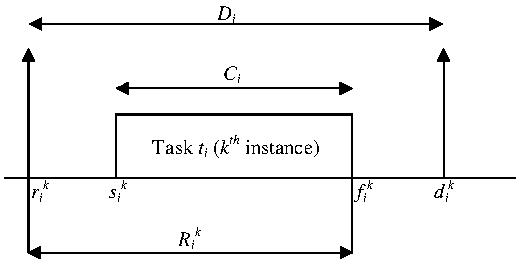
\includegraphics{figures/taskmodel}
\caption{Parameters of a real-time task.}
\label{fig:taskmodel}
\end{figure} 

Real-time systems can be classified based on the impact of missing deadlines. Hard real-time systems are systems where all deadlines must be met. Violating this constraint leads to the failure of the system and may result in a great loss such as serious injuries, threatening human life, or damaging the surroundings. Soft real-time systems can tolerate some deadlines to be missed but the quality of the result degrades consequently. Firm real-time systems allow few deadlines to be missed but if a task's deadline is missed, its result is no more useful. We consider that HiL simulation falls within the category of firm real-time systems. In fact, in order to have correct HiL results, deadlines must be met. If a task misses its deadline, it produces erroneous results and probably causes the failure of the system but the consequences are not as catastrophic and harming as in the case of hard real-time systems.   

Many different real-time scheduling algorithms have been proposed in the literature but they are all based on the same idea, tasks are assigned priorities and then scheduled in an order following their priorities. We distinguish between fixed priorities which do not change during the execution and dynamic priorities which may be changed by the scheduler during the execution. Also, as in other kinds of scheduling problems, real-time scheduling algorithms can be classified into offline/online and preemptive/non preemptive algorithms.

The main goal of scheduling in real-time systems is to satisfy the different timing constraints of the tasks. Schedulability tests are performed to check whether the tasks can be scheduled using a given scheduling algorithm in such a way to satisfy all the requirements. The schedulability test verifies if the utilization or the density of the processor, defined below, when it executes the set of tasks under test, is within a least upper bound. For a set of $n$ independent periodic tasks, the utilization factor and density, when a preemptive scheduling algorithm is used, are respectively:

\begin{equation}
U = \sum_{i=1}^{n}\frac{C_i}{T_i}
\end{equation}

\begin{equation}
\Delta = \sum_{i=1}^{n}\frac{C_i}{D_i}
\end{equation}
The most known real-time scheduling algorithms are the following:

\begin{itemize}
\item Fixed priorities
\begin{itemize}
\item Rate Monotonic (RM): Tasks are assigned priorities inversely proportional to their periods. A set of tasks is schedulable by RM if: $U \leq n(2^{\frac{1}{n}}-1)$, $D_i = T_i$. 
\item Deadline Monotonic (DM): Tasks are assigned priorities inversely proportional to their relative deadlines. Tasks are schedulable using DM if: $\Delta \leq n(2^{\frac{1}{n}}-1)$, $D_i \leq T_i$. 
\end{itemize}
\item Dynamic priorities
\begin{itemize}
\item Earliest Deadline First (EDF): Priorities of tasks are inversely proportional to their absolute deadlines. The priority of a task is fixed for one instance but may change from one instance to another. EDF can schedule a set of tasks if and only if: $U \leq 1, D_i = T_i$.
\item Least Laxity First (LLF): Priorities of tasks are inversely proportional to their laxities. The priority may change for the same instance and from one instance to another. The schedulability test is the same as for EDF.
\end{itemize}
\end{itemize}
 For multiprocessor real-time scheduling, there exist two principal approaches:

\begin{itemize}
\item Global scheduling: Each task can be scheduled on any processor. the scheduler is responsible for migrating the tasks between the processors.
\item Partitioned scheduling: The tasks are partitioned into groups, each of which is allocated to one processor. Each processor has a single-processor scheduler. 
\end{itemize}
Global multiprocessor scheduling has significant overhead due to the migration cost. That is the reason why partitioned scheduling is usually used in hard real-time systems. Partitioning and allocating a set of tasks is equivalent to the "Bin Packing" problem which is NP-hard and heuristics are therefore used. 

Assuming the tasks are sorted in a list and that processors are organized in a certain order, the most known heuristics that can be used to allocate a set of tasks to multiple processors are:

\begin{itemize}
\item First Fit (FF): A task is tested on all cores and for each task the test starts from the first core. The task is allocated to the first found core that can schedule it. A task is schedulable on a given core if by allocating it to this core the condition $(U\leq1)$ is valid where $U$ is the utilization of the core.
\item Next Fit (NF): Similar to FF but the search of the core that can schedule the task does not start always from the first one. After allocating a task to a core, the core search for the next task starts from the next core.
\item Best Fit (BF): Test the task on all cores and allocate it to the one that gives the minimum of $U$.
\item Worst Fit (WF): Allocate the task to the core that gives the maximum of $U$.
\end{itemize}
  
\section{Parallelization of Co-simulation}

The more accurate is a simulation of a system, the more reliable is the assessment of its behavior. The numerical accuracy can be improved in different ways, for instance, by choosing a small integration step size. However, this means that more computations are performed and thus the computation load becomes large decreasing the simulation performance. An important challenge faced by the developers and the users of simulation tools is to achieve a good simulation performance while maintaining an acceptable simulation accuracy. 

The performance of a simulation can be significantly improved through parallel execution. In this scope, different approaches for the parallelization of simulations have been porposed in the literature. In this section we briefly review some of the approaches for the parallelization of simulation that are found in the literature. We present also some of the available simulation tools that support parallel simulations.

\subsection{Methods}

In order to achieve simulation acceleration through parallel execution, different approaches are possible and were already explored. The parallelization approaches can be classified into three categories based on the level at which the parallelization is intorduced.

\subsubsection{Parallelization across the method}
In this category, we find approaches that seek to parallelize the integration method. For instance, a multi-satge solver requires several computations within one integration step and it is possible to perform multiple computations within one step in parallel. Such approach is studied in \cite{iserles:1990} by proposing a theoretical framework for parallelization of Runge-Kutta methods. Another approach consists in parallelizing operations on vectors for ODEs resolution like in the PVODE solver \cite{byrne:1999} implemented using MPI. 

In \cite{elmqvist:2015}, the authors propose a method for parallelization of modelica programs on CUDA-enabled GPUs. The proposed method relies on marking the functions to be executed on the GPU by identifying patterns that are GPU suitable such as loops. These functions are then automatically translated into GPU code. In \cite{Gebremedhin2012}, ParModelica, an algorithmic extension to Modelica is proposed. This extension is based on OpenCL and allows stating the parallelism using special declarations in the code. An approach for automatic parallelization of equations on many-core platforms is proposed in \cite{elmqvist:2014}. This approach organizes the equations into a set of layers containing each a number of sections that can be executed in parallel and computes a static schedule for their execution. In \cite{clauberg:2012} an approach for the parallelization of multi-body simulations on shared memory multiprocessors is processors. This approach uses math-kernel libraries and OpenMP to parallelize matrix operations.

\subsubsection{Parallelization across the time}

A simulation can be parallelized across the time steps. Examples of such approach are the Parreal algorithm \cite{lions:2001}, the Parallel Implicit Time-Integrator (PITA) \cite{farhat:2003}, and the Parallel Full Approximation Scheme in Space and Time (PFASST) \cite{emmett:2012}. These methods divide the time domain into a two-level grid. A solution is evaluated in parallel over a fine time grid to improve a solution obtained sequentially over a coarse time grid.
\subsubsection{Parallelization across the system}

Finally, a simulation can be parallelized across the system, i.e. the equations of the simulation are solved in parallel. A well known approach that parallelizes across the system is Waveform Relaxation (WR) \cite{lelarasmee:1982}, initially introduced for the simulation of large scale integrated circuits. The WR method breaks down the system into coupled subsystems of equations and computes the waveform, i.e. the solution, of each subsystem over a given time interval while fixing the waveforms of the other subsystems. The parallelization is made possible by computing the waveforms of several subsystems in parallel. 

Transmission Line Modeling (TLM) \cite{hui:1990} is a method that allows the decoupling and the parallelization of models by representing them using transmission line graphs such that decoupling points are chosen where variables change slowly because the models are considered to be connected by constants at these points. The approaches presented in \cite{sjolund:2010,braun:2012} are based on the TLM method. 

Co-simulation is naturally adapted to parallelization across the system. In fact, as shown in \cite{Benkhaled_A_2012_ECOSM}, splitting a model into several FMUs, by isolating discontinuities, may reduce the simulation time, even in the case of a sequential execution. In \cite{benkhaled:2014} the Refined CO-SIMulation (RCOSIM) approach is presented. It consists in using each FMU information on input/output causality to build a graph, with an increased granularity and then exploiting the potential parallelism by using a heuristic to build an offline multi-core schedule.

\subsection{Tools}

More and more simulation tools are now endowed with parallel execution capabilities. However, it should be noted that some of these tools adopt parallelization approaches that do not target the numerical part of the simulation. For instance, the Parallel Computing Toolbox in MATLAB allows launching multiple Simulink simulations of the same model in parallel on a desktop multi-core computer or a cluster. These are separate independent simulations of the same model. Thus, this feature does not correspond to the focus of this thesis, i.e. the parallelization of the numerical computations of a simulation. Also, Simulink provides an execution mode known as Rapid Accelerator Mode which consists in creating a standalone executable of the model and the solver. Simulink runs in one process and this executable runs in another process on a multi-core processor. Again, although this approach may improve the performance of the simulation, it does not lie within the scope of the thesis.

The Dymola tool enables automatic parallelization of equation resolution. The prallelization approach of Dymola is detailed in \cite{elmqvist:2014}. Amesim allows launching multiple simulations in parallel, for example to run a model with different parameters. It has also the capability of partitioning models and executing them on multi-core processors. The TLM method, presented above, is integrated in the Hopsan tool. Finally, MBSim parallelizes matrix and vector operations as described in \cite{clauberg:2012}. 